\normalfalse \difficiletrue \tdifficilefalse
\correctiontrue

%\UPSTIidClasse{11} % 11 sup, 12 spé
%\newcommand{\UPSTIidClasse}{12}

\exer{Mouvement RR 3D  $\star\star$ \label{B2:13:07}}
\setcounter{question}{0}\marginnote{\UPSTIcompetence[2]{C2-05}
\UPSTIcompetence[2]{B2-13}}
\index{Compétence C2-05}
\index{Compétence B2-13}
\index{Mécanisme à 2 rotations 3D}
\ifcorrection
\else
\marginnote{\textbf{Pas de corrigé pour cet exercice.}}
\fi

\ifprof
\else
Soit le mécanisme suivant. On a $\vect{AB}=R\vect{i_1}$ et $\vect{BC}=\ell\vect{i_2}+r\vect{j_2}$. On note $R+\ell=L = \SI{20}{mm}$ et $r=\SI{10}{mm}$.
\begin{center}
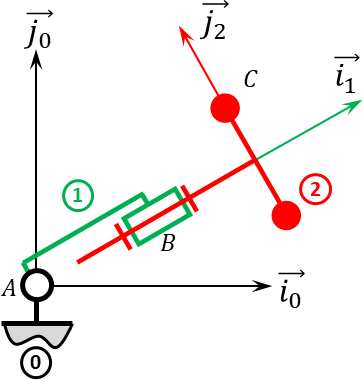
\includegraphics[width=.8\linewidth]{07_RR3D_01}
\end{center}
\fi


\ifprof
\else
\marginnote{
\begin{solution}
\begin{enumerate}
\item .
\item $x_C(t)= \left(R+\ell\right)\cos\theta  - r\cos\varphi  \sin\theta$, 
$y_C(t)= \left(R+\ell\right)\sin\theta  + r\cos\varphi \cos\theta$, 
$z_C(t)=  r\sin\varphi$.
\end{enumerate}
\end{solution}
Corrigé  voir \ref{B2:13:07}.}
\fi

\question{Donner l'ensemble des positions accessibles par le point $C$.}
\ifprof
Ça ressemble à un tore, mais c'est pas vraiment un tore :) (aussi bien l'intérieur que l'extérieur...)...
\else
\fi

\question{Donner l'équation du mouvement du point $C$ dans le mouvement de \textbf{2} par rapport à \textbf{0}.}
\ifprof ~\\
On a $\vect{AC}=\vect{AB}+\vect{BC} = R\vect{i_1} + \ell\vect{i_2}+r\vect{j_2}$. 
Soit $\vect{AC} = \left(R+\ell\right)\left(\cos\theta\vi{0} + \sin\theta\vj{0}\right)  + r\left(\cos\varphi \vj{1}+\sin\varphi \vk{1}\right)$  $= \left(R+\ell\right)\left(\cos\theta\vi{0} + \sin\theta\vj{0}\right)  + r\left(\cos\varphi \left(  \cos\theta\vj{0} - \sin\theta\vi{0}\right)+\sin\varphi \vk{0}\right)$.

On a donc :
$\left\{
\begin{array}{l}
x_C(t)= \left(R+\ell\right)\cos\theta  - r\cos\varphi  \sin\theta\\
y_C(t)= \left(R+\ell\right)\sin\theta  + r\cos\varphi \cos\theta \\
z_C(t)=  r\sin\varphi \\
\end{array}
\right.
$ dans le repère $\repere{A}{i_0}{j_0}{k_0}$.
\else
\fi

